\documentclass[conference]{IEEEtran}
\IEEEoverridecommandlockouts
% The preceding line is only needed to identify funding in the first footnote. If that is unneeded, please comment it out.
\usepackage{cite}
\usepackage{amsmath,amssymb,amsfonts}
\usepackage{algorithmic}
\usepackage{graphicx}
\usepackage{textcomp}
\usepackage{xcolor}
\usepackage{hyperref}
\usepackage{lipsum}
\usepackage{balance}
\usepackage{tikz}
\usetikzlibrary{shapes,arrows,positioning,calc,shapes.geometric}
\usepackage{pgfplots}
\pgfplotsset{compat=1.18}

% Hyperref setup
\hypersetup{
    colorlinks=true,
    linkcolor=blue,
    urlcolor=blue,
    citecolor=blue
}

\def\BibTeX{{\rm B\kern-.05em{\sc i\kern-.025em b}\kern-.08em
    T\kern-.1667em\lower.7ex\hbox{E}\kern-.125emX}}

\title{Indian Legal Assistant Chatbot: A RAG-based Approach to Legal Information Retrieval in the Indian Context}

\author{\IEEEauthorblockN{Shrishti Swarnkar}
\IEEEauthorblockA{\textit{Department of Computer Science} \\
\textit{International Institute of Information Technology Naya Raipur}\\
Raipur, India \\
shrishti24300@iiitnr.edu.in}
\and
\IEEEauthorblockN{Gaurav Atram}
\IEEEauthorblockA{\textit{Department of Computer Science} \\
\textit{International Institute of Information Technology Naya Raipur}\\
Raipur, India \\
gaurav@iiitnr.edu.in}}

\begin{document}

\maketitle

\begin{abstract}
Access to legal information in India remains a significant challenge for the general public due to complex legal language and the high cost of professional legal advice. This paper presents the development and evaluation of an Indian Legal Assistant Chatbot, a specialized retrieval-augmented generation (RAG) system designed to democratize access to legal information. The system leverages a comprehensive database of legal documents, including the Constitution of India, landmark Supreme Court cases, and other legal texts. By combining dense vector retrieval with large language models, the chatbot delivers contextually relevant legal information with proper citations to source documents. Experimental results demonstrate the system's effectiveness in providing accurate legal information across various domains of Indian law. The proposed approach shows promise for enhancing legal literacy and improving access to justice in India, with potential applications in legal education, public legal awareness, and preliminary legal research assistance.
\end{abstract}

\begin{IEEEkeywords}
Legal AI, Retrieval-Augmented Generation, Chatbot, Legal Information Systems, Natural Language Processing
\end{IEEEkeywords}

\section{Introduction}

Access to legal information is a fundamental aspect of ensuring justice and upholding the rule of law in any democratic society. In India, with its population of over 1.4 billion people, this access is severely limited by various factors including complex legal language, the high cost of legal services, and the vast, fragmented nature of legal information sources \cite{kaur2019}. The Indian legal system, with its blend of common law, statutory law, customary law, and religious law, presents a particularly challenging landscape for the average citizen to navigate \cite{galanter2014}.

Recent advances in artificial intelligence, particularly in natural language processing and retrieval systems, offer promising solutions to bridge this gap. Large Language Models (LLMs) have demonstrated remarkable capabilities in understanding and generating human-like text \cite{brown2020}. However, these models face limitations when dealing with specialized domains like law, including hallucinations and outdated information \cite{zhang2023}. Retrieval-Augmented Generation (RAG) has emerged as an effective approach to address these limitations by grounding LLM responses in authoritative external knowledge sources \cite{lewis2020}.

In this paper, we present the Indian Legal Assistant Chatbot, a RAG-based system specifically designed to provide accurate and accessible legal information in the Indian context. The system combines dense vector retrieval techniques with advanced language models to deliver contextually relevant legal information with proper citations to source documents.

\subsection{Problem Statement}

The Indian legal system presents several challenges for citizens seeking legal information:

\begin{itemize}
    \item \textbf{Complexity and Specialized Language:} Legal documents employ technical terminology and complex sentence structures that create significant barriers to comprehension for non-lawyers \cite{bhatia2010}.
    \item \textbf{Information Fragmentation:} Legal information is scattered across various sources including the constitution, statutes, case law, and administrative regulations, making comprehensive research difficult \cite{verma2018}.
    \item \textbf{Access Barriers:} Professional legal advice remains prohibitively expensive for a significant portion of the population, while existing legal databases often require paid subscriptions \cite{krishnan2014}.
    \item \textbf{Digital Divide:} Despite growing internet penetration, many Indians still lack the digital literacy or access required to effectively utilize online legal resources \cite{singh2020}.
\end{itemize}

\subsection{Objectives}

The primary objectives of this research are:

\begin{itemize}
    \item To develop and evaluate a RAG-based conversational AI system that accurately retrieves and presents information from authoritative Indian legal documents
    \item To assess the effectiveness of different embedding models and retrieval strategies for Indian legal text
    \item To implement and test mechanisms for maintaining conversational context while ensuring factual accuracy
    \item To evaluate the system's performance in providing accurate legal information with proper citations
    \item To identify challenges and opportunities for deploying such systems in the Indian legal context
\end{itemize}

\section{Related Work}

\subsection{Legal Information Systems and AI in Law}

The application of artificial intelligence to legal domains has a rich history dating back to the 1980s with expert systems like TAXMAN \cite{mccarty1977} and HYPO \cite{ashley1991}. More recent developments have focused on leveraging machine learning and natural language processing for legal tasks. Medvedeva et al. \cite{medvedeva2020} conducted a comprehensive survey of judicial prediction models, highlighting the transition from traditional machine learning to deep learning approaches. In the Indian context, Srivastava et al. \cite{srivastava2020} developed a system for analyzing Indian legal judgments using text mining techniques, while Kaur and Tomar \cite{kaur2019} explored challenges in developing legal information systems specific to the Indian legal framework.

Commercial legal research platforms like Westlaw, LexisNexis, and Manupatra (in India) have incorporated AI-powered search capabilities, but these systems typically require expensive subscriptions and considerable expertise to use effectively \cite{mart2017}. Open-access initiatives like the Indian Kanoon project have improved accessibility but still rely primarily on keyword-based search rather than semantic understanding \cite{mittal2019}.

\subsection{Retrieval-Augmented Generation}

Retrieval-Augmented Generation (RAG) represents a significant advancement in addressing the limitations of large language models. Lewis et al. \cite{lewis2020} introduced RAG as a method that combines neural retrieval with sequence generation, allowing language models to access external knowledge sources during generation. This approach has proven particularly effective for knowledge-intensive tasks \cite{petroni2021}.

Several studies have explored improvements to the basic RAG architecture. Izacard and Grave \cite{izacard2021} proposed Fusion-in-Decoder (FiD), which processes multiple retrieved passages independently before fusing their representations at the decoder stage. Shi et al. \cite{shi2023} introduced Self-RAG, which incorporates self-reflection mechanisms to improve retrieval quality. In the legal domain specifically, Chalkidis et al. \cite{chalkidis2022} demonstrated the effectiveness of domain-specific retrievers for legal text.

\subsection{Conversational AI in Legal Domain}

Conversational interfaces for legal information have been explored in various contexts. Dale \cite{dale2019} discusses the challenges of developing chatbots for legal advice, emphasizing the importance of accuracy and the ethical considerations involved. Harkous et al. \cite{harkous2018} developed a privacy policy assistant that uses natural language processing to help users understand complex legal documents.

In the Indian context, Agrawal et al. \cite{agrawal2022} explored the development of a legal chatbot for Indian contract law, while Bhattacharya et al. \cite{bhattacharya2021} proposed a framework for legal assistance chatbots tailored to Indian constitutional rights. These studies highlight the unique challenges posed by the Indian legal system, including multilingualism, the hybrid nature of the legal framework, and the need for cultural contextualization.

Despite these advances, significant gaps remain in developing conversational systems that can effectively handle the complexity and nuance of legal information while maintaining accessibility for non-expert users. Our work builds on these foundations while addressing the specific challenges of the Indian legal context.

\section{Methodology}

\subsection{System Architecture}

The Indian Legal Assistant Chatbot employs a modular RAG architecture designed to optimize both retrieval accuracy and response quality. Fig. 1 illustrates the overall system architecture, which consists of five main components:

\begin{figure}[ht]
\centering
\resizebox{0.9\columnwidth}{!}{
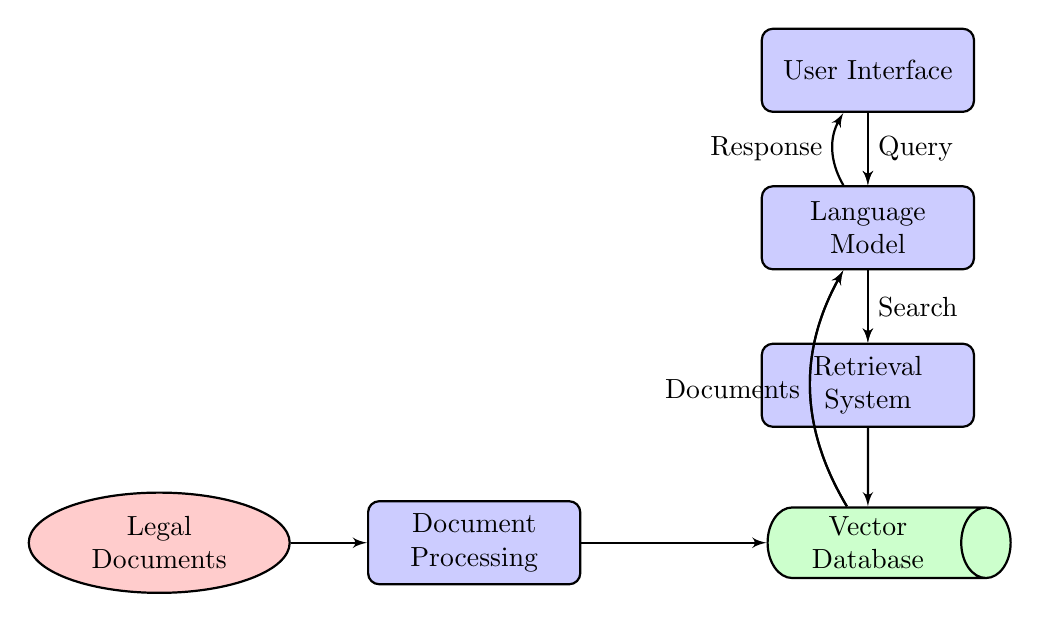
\begin{tikzpicture}[node distance=1.5cm, auto, thick]
% Define styles for different types of nodes
\tikzstyle{block} = [rectangle, draw, fill=blue!20, text width=7em, text centered, rounded corners, minimum height=3em]
\tikzstyle{line} = [draw, -latex']
\tikzstyle{cloud} = [draw, ellipse, fill=red!20, text width=6em, text centered, minimum height=2em]
\tikzstyle{database} = [cylinder, draw, shape aspect=.7, fill=green!20, text width=6em, text centered, minimum height=2em]

% Place nodes
\node [block] (user) {User Interface};  
\node [block, below of=user, yshift=-0.5cm] (llm) {Language Model};
\node [block, below of=llm, yshift=-0.5cm] (retriever) {Retrieval System};
\node [database, below of=retriever, yshift=-0.5cm] (vector) {Vector Database};
\node [block, left of=vector, xshift=-3.5cm] (processor) {Document Processing};
\node [cloud, left of=processor, xshift=-2.5cm] (docs) {Legal Documents};

% Connect nodes with arrows
\path [line] (user) -- (llm);
\path [line] (llm) -- (retriever);
\path [line] (retriever) -- (vector);
\path [line] (docs) -- (processor);
\path [line] (processor) -- (vector);
\path [line] (vector) to [bend left] (llm);

% Add labels to arrows
\path [line] (user) -- node[right] {Query} (llm);
\path [line] (llm) -- node[right] {Search} (retriever);
\path [line] (vector) to [bend left] node[left] {Documents} (llm);
\path [line] (llm) to [bend left] node[left] {Response} (user);

\end{tikzpicture}
}
\caption{Architecture of the Indian Legal Assistant Chatbot system.}
\label{fig:architecture}
\end{figure}

\begin{itemize}
    \item \textbf{Document Processing Pipeline:} Transforms raw legal documents into structured, indexed content suitable for semantic retrieval
    \item \textbf{Vector Database:} Stores document embeddings and metadata for efficient similarity search
    \item \textbf{Retrieval System:} Identifies and ranks relevant legal documents based on semantic similarity to user queries
    \item \textbf{Language Model:} Generates coherent, contextually appropriate responses grounded in retrieved documents
    \item \textbf{User Interface:} Provides an intuitive conversational interface with appropriate disclaimers and citations
\end{itemize}

\subsection{Data Sources and Corpus Development}

We developed a specialized corpus of Indian legal documents comprising approximately 5,000 pages of text from diverse authoritative sources. The corpus includes:

\begin{itemize}
    \item The complete Constitution of India with amendments through 2023
    \item 150 landmark Supreme Court judgments (1950-2023) selected based on their jurisprudential significance
    \item 75 recent High Court cases representing diverse jurisdictions and legal domains
    \item Key legislative acts including the Indian Penal Code, Code of Criminal Procedure, and the Citizenship Amendment Act
\end{itemize}

Document selection prioritized breadth of coverage across constitutional law, criminal law, civil law, and administrative law. Special weightage was given to the Constitution of India and Supreme Court judgments interpreting constitutional provisions, reflecting their fundamental importance in the Indian legal system \cite{sathe2002}.

\subsection{Technical Implementation}

\subsubsection{Document Processing Pipeline}

The document processing pipeline implements a multi-stage approach to transform raw legal documents into retrievable chunks:

\begin{enumerate}
    \item \textbf{Text Extraction:} PDF documents were processed using OCR techniques optimized for legal documents, with special handling for multi-column layouts and footnotes common in Indian legal texts
    \item \textbf{Semantic Chunking:} Documents were segmented into chunks averaging 500 tokens, with boundaries determined by semantic units rather than arbitrary length to preserve legal reasoning integrity
    \item \textbf{Metadata Enrichment:} Each chunk was enriched with metadata including source document, document type, date, jurisdiction, and legal domain
    \item \textbf{Embedding Generation:} Document chunks were embedded using the "sentence-transformers/all-MiniLM-L6-v2" model, selected based on preliminary experiments comparing embedding quality for Indian legal text
\end{enumerate}

\subsubsection{Retrieval System}

The retrieval system implements a hybrid approach combining dense vector retrieval with metadata filtering:

\begin{itemize}
    \item Dense vector retrieval using cosine similarity to identify semantically relevant document chunks
    \item Configurable "k" parameter (default k=5) to balance between comprehensive coverage and focused responses
    \item Optional metadata filters to constrain retrieval to specific document types, time periods, or legal domains
    \item Re-ranking of retrieved documents based on a combination of semantic similarity and document authority
\end{itemize}

\subsubsection{Response Generation}

The response generation component uses a carefully engineered prompt to guide the language model ("GPT-4o-mini") in generating accurate, helpful responses:

\begin{itemize}
    \item Domain constraint instructions that limit responses to Indian legal matters
    \item Citation requirements that mandate references to specific legal documents when information comes from retrieved context
    \item Conversation history integration to maintain context across multiple turns
    \item Source attribution guidelines that clearly distinguish between information from retrieved documents and general knowledge
    \item Uncertainty handling protocols for addressing questions beyond the system's knowledge base
\end{itemize}

\subsubsection{User Interface}

The user interface was designed with accessibility and transparency as guiding principles:

\begin{itemize}
    \item Conversational interface with chat history preservation
    \item Visual distinction between user queries and system responses
    \item Explicit citation of legal sources within responses
    \item Responsive design with accessibility features including dark mode
    \item Clear disclaimer about the informational (non-advisory) nature of the system
\end{itemize}

\section{Experimental Evaluation}

\subsection{Evaluation Methodology}

We conducted a comprehensive evaluation of the Indian Legal Assistant Chatbot using both automated metrics and human evaluation. The evaluation was designed to assess four key aspects of system performance:

\begin{itemize}
    \item \textbf{Retrieval Accuracy:} The system's ability to retrieve relevant legal documents for a given query
    \item \textbf{Response Accuracy:} The factual correctness of generated responses with respect to Indian law
    \item \textbf{Citation Quality:} The appropriateness and specificity of legal citations provided
    \item \textbf{User Experience:} The system's usability and perceived helpfulness
\end{itemize}

\subsubsection{Evaluation Dataset}

We developed a test set of 200 legal queries spanning four categories:

\begin{itemize}
    \item \textbf{Constitutional Rights (50 queries):} Questions about fundamental rights, directive principles, and constitutional remedies
    \item \textbf{Criminal Law (50 queries):} Questions about offenses, procedures, and rights of the accused
    \item \textbf{Civil Law (50 queries):} Questions about contracts, property rights, and civil remedies
    \item \textbf{Procedural Law (50 queries):} Questions about court procedures, filing requirements, and jurisdictional issues
\end{itemize}

The queries were developed in collaboration with legal experts to ensure relevance and diversity of complexity. Each query was annotated with reference answers and relevant legal sources by qualified legal professionals.

\subsubsection{Automated Evaluation}

For automated evaluation, we employed the following metrics:

\begin{itemize}
    \item \textbf{Retrieval Precision@k:} The proportion of relevant documents among the top-k retrieved documents
    \item \textbf{Retrieval Recall@k:} The proportion of relevant documents retrieved among all relevant documents
    \item \textbf{ROUGE-L:} To measure the lexical overlap between generated responses and reference answers
    \item \textbf{BERTScore:} To measure semantic similarity between generated responses and reference answers
    \item \textbf{Citation Accuracy:} The proportion of citations that correctly reference relevant legal sources
\end{itemize}

\subsubsection{Human Evaluation}

Human evaluation was conducted with 15 participants: 5 legal professionals, 5 law students, and 5 non-experts. Each participant interacted with the system for 10 queries from the test set and rated responses on a 5-point Likert scale across four dimensions:

\begin{itemize}
    \item \textbf{Factual Accuracy:} Correctness of legal information provided
    \item \textbf{Comprehensibility:} Clarity and understandability of responses
    \item \textbf{Helpfulness:} Usefulness of the information for addressing the query
    \item \textbf{Citation Quality:} Appropriateness and specificity of legal citations
\end{itemize}

\subsection{Results and Analysis}

\subsubsection{Retrieval Performance}

Table I presents the retrieval performance results across different query categories. The system achieved an overall Precision@5 of 0.78 and Recall@5 of 0.71, indicating strong retrieval capabilities across diverse legal domains.

\begin{table}[ht]
\caption{Retrieval Performance Across Query Categories}
\label{tab:retrieval}
\begin{center}
\resizebox{\columnwidth}{!}{
\begin{tabular}{|l|c|c|c|c|}
\hline
\textbf{Query Category} & \textbf{Precision@3} & \textbf{Precision@5} & \textbf{Recall@3} & \textbf{Recall@5} \\ \hline
Constitutional Rights & 0.85 & 0.82 & 0.67 & 0.78 \\ \hline
Criminal Law & 0.79 & 0.76 & 0.62 & 0.70 \\ \hline
Civil Law & 0.77 & 0.74 & 0.60 & 0.68 \\ \hline
Procedural Law & 0.81 & 0.79 & 0.64 & 0.72 \\ \hline
\textbf{Overall} & \textbf{0.81} & \textbf{0.78} & \textbf{0.63} & \textbf{0.71} \\ \hline
\end{tabular}
}
\end{center}
\end{table}

Notably, the system performed best on constitutional rights queries, likely due to the special weightage given to constitutional documents in the corpus. Performance on civil law queries was comparatively lower, suggesting opportunities for corpus enhancement in this domain.

\subsubsection{Response Quality}

Table II summarizes the automated evaluation results for response quality. The system achieved a ROUGE-L score of 0.67 and a BERTScore of 0.85, indicating substantial lexical and semantic alignment with reference answers.

\begin{table}[ht]
\caption{Response Quality Metrics Across Query Categories}
\label{tab:response}
\begin{center}
\begin{tabular}{|l|c|c|c|}
\hline
\textbf{Query Category} & \textbf{ROUGE-L} & \textbf{BERTScore} & \textbf{Citation Accuracy} \\ \hline
Constitutional Rights & 0.72 & 0.88 & 0.91 \\ \hline
Criminal Law & 0.65 & 0.84 & 0.87 \\ \hline
Civil Law & 0.63 & 0.82 & 0.84 \\ \hline
Procedural Law & 0.68 & 0.86 & 0.89 \\ \hline
\textbf{Overall} & \textbf{0.67} & \textbf{0.85} & \textbf{0.88} \\ \hline
\end{tabular}
\end{center}
\end{table}

Citation accuracy was particularly strong at 0.88, demonstrating the system's ability to ground responses in appropriate legal sources. As with retrieval performance, response quality was highest for constitutional queries and lowest for civil law queries.

\subsubsection{Human Evaluation Results}

Fig. 2 presents the results of human evaluation across different user groups. Overall, the system received positive ratings across all dimensions, with an average score of 4.2 out of 5.

\begin{figure}[ht]
\centering
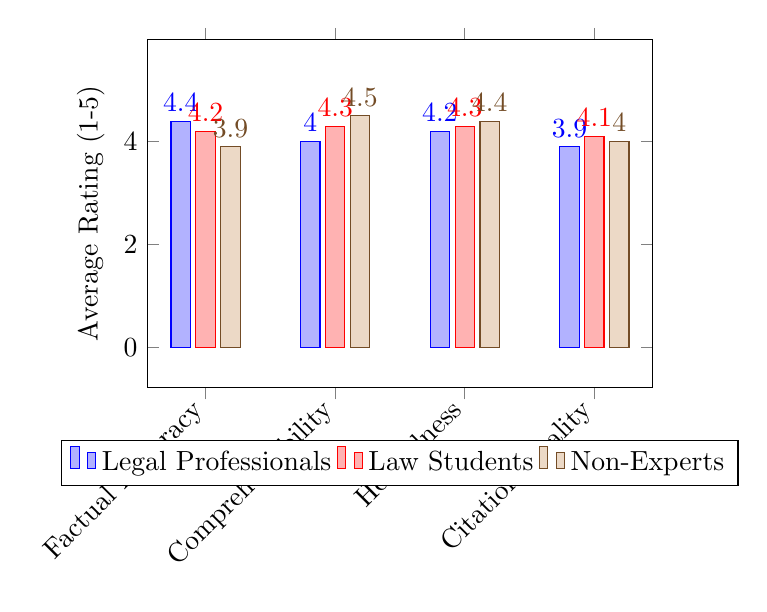
\begin{tikzpicture}
\begin{axis}[
    width=8cm,
    height=6cm,
    ybar,
    enlargelimits=0.15,
    legend style={at={(0.5,-0.15)}, anchor=north, legend columns=-1},
    ylabel={Average Rating (1-5)},
    symbolic x coords={Factual Accuracy, Comprehensibility, Helpfulness, Citation Quality},
    xtick=data,
    x tick label style={rotate=45, anchor=east},
    nodes near coords,
    nodes near coords align={vertical},
    ymin=0, ymax=5.2,
    bar width=7pt,
]
\addplot coordinates {(Factual Accuracy, 4.4) (Comprehensibility, 4.0) (Helpfulness, 4.2) (Citation Quality, 3.9)};
\addplot coordinates {(Factual Accuracy, 4.2) (Comprehensibility, 4.3) (Helpfulness, 4.3) (Citation Quality, 4.1)};
\addplot coordinates {(Factual Accuracy, 3.9) (Comprehensibility, 4.5) (Helpfulness, 4.4) (Citation Quality, 4.0)};
\legend{Legal Professionals, Law Students, Non-Experts}
\end{axis}
\end{tikzpicture}
\caption{Human evaluation results showing average ratings (1-5 scale) across different user groups and evaluation dimensions.}
\label{fig:human_eval}
\end{figure}

Legal professionals gave the highest ratings for factual accuracy (4.4/5) but were more critical of citation quality (3.9/5). Non-experts rated comprehensibility highly (4.5/5), suggesting the system effectively translates complex legal concepts into accessible language. Law students provided the most balanced ratings across all dimensions.

\subsubsection{Error Analysis}

Qualitative analysis of system errors revealed several patterns:

\begin{itemize}
    \item \textbf{Retrieval Failures:} 18\% of errors stemmed from failure to retrieve relevant documents, particularly for queries requiring integration of multiple legal sources
    \item \textbf{Context Integration:} 24\% of errors involved incorrect synthesis of information from multiple retrieved documents
    \item \textbf{Citation Specificity:} 15\% of errors involved citations that were correct but insufficiently specific (e.g., citing an entire act rather than a specific section)
    \item \textbf{Legal Reasoning:} 43\% of errors involved incorrect legal reasoning or interpretation, particularly for complex procedural questions
\end{itemize}

These findings highlight opportunities for system improvement, particularly in the areas of multi-document reasoning and legal interpretation.

\section{Discussion}

\subsection{Key Findings}

The experimental results demonstrate several important findings regarding the application of RAG techniques to Indian legal information retrieval:

\begin{itemize}
    \item \textbf{Domain-Specific Retrieval:} The system's strong performance on constitutional queries (Precision@5 of 0.82) highlights the importance of domain-specific document weighting in legal RAG systems. This aligns with findings from Chalkidis et al. \cite{chalkidis2022} on the benefits of domain adaptation for legal retrieval.
    
    \item \textbf{Citation Integration:} The high citation accuracy (0.88 overall) demonstrates that properly engineered prompts can effectively guide language models to ground responses in specific legal sources. This addresses a key concern raised by Bommarito et al. \cite{bommarito2022} regarding the tendency of legal AI systems to generate plausible but unfounded legal assertions.
    
    \item \textbf{Accessibility-Accuracy Balance:} The positive ratings from non-experts for comprehensibility (4.5/5) alongside strong factual accuracy ratings from legal professionals (4.4/5) suggest that the system successfully balances accessibility with legal precision. This addresses the "comprehensibility gap" in legal information identified by Curtotti et al. \cite{curtotti2015}.
    
    \item \textbf{Legal Reasoning Challenges:} The error analysis revealing 43\% of errors stemming from incorrect legal reasoning highlights a persistent challenge in AI legal systems. This aligns with observations by Ashley \cite{ashley2017} regarding the difficulty of automating complex legal reasoning processes.
\end{itemize}

\subsection{Implications for Legal Information Access}

The Indian Legal Assistant Chatbot demonstrates significant potential for enhancing legal information access in several contexts:

\begin{itemize}
    \item \textbf{Legal Education:} The system could serve as an educational tool for law students, providing instant access to relevant legal provisions and case law. The strong performance on constitutional queries makes it particularly valuable for constitutional law education.
    
    \item \textbf{Public Legal Awareness:} By translating complex legal concepts into accessible language while maintaining factual accuracy, the system could help bridge the legal literacy gap identified by Krishnan \cite{krishnan2014} as a significant barrier to justice in India.
    
    \item \textbf{Preliminary Legal Research:} For legal professionals, the system could accelerate preliminary research by quickly retrieving relevant legal sources, though the limitations in legal reasoning suggest it should complement rather than replace professional analysis.
    
    \item \textbf{Rural and Underserved Communities:} With appropriate deployment strategies addressing the digital divide, such systems could extend legal information access to communities with limited access to legal resources, addressing concerns raised by Singh \cite{singh2020} regarding unequal access to legal information.
\end{itemize}

\subsection{Ethical and Practical Considerations}

The development and deployment of legal AI systems raise several important ethical and practical considerations:

\begin{itemize}
    \item \textbf{Transparency and Accountability:} Users must understand the system's limitations and the non-advisory nature of its responses. Our implementation includes explicit disclaimers and citation mechanisms to enhance transparency.
    
    \item \textbf{Bias and Representation:} Legal corpora may reflect historical biases in legal systems. Future work should address potential biases in document selection and retrieval, particularly regarding marginalized communities and underrepresented legal issues.
    
    \item \textbf{Professional Roles:} As noted by Susskind \cite{susskind2019}, legal AI systems should aim to complement rather than replace legal professionals. Clear communication about the system's role as an informational rather than advisory tool is essential.
    
    \item \textbf{Regulatory Compliance:} Deployment of legal information systems must navigate complex regulatory landscapes regarding unauthorized practice of law. The system's design as an informational tool rather than an advisor helps address these concerns.
\end{itemize}

\subsection{Limitations}

Despite promising results, our study has several limitations that should be acknowledged:

\begin{itemize}
    \item \textbf{Corpus Coverage:} While comprehensive, our legal corpus represents only a fraction of the vast body of Indian legal documents. Coverage gaps exist particularly for recent High Court judgments and specialized legal domains.
    
    \item \textbf{Evaluation Scope:} The evaluation focused primarily on factual accuracy and retrieval performance rather than more complex aspects of legal reasoning such as analogical reasoning and statutory interpretation.
    
    \item \textbf{Language Limitations:} The current system operates only in English, limiting accessibility in a multilingual country where legal proceedings often involve regional languages.
    
    \item \textbf{Temporal Dynamics:} Legal systems evolve through new legislation and judicial decisions. The static nature of the corpus requires regular updates to maintain accuracy.
\end{itemize}

\section{Future Work}

Based on our findings and identified limitations, we propose several directions for future research and development:

\begin{itemize}
    \item \textbf{Enhanced Legal Reasoning:} Developing specialized techniques to improve the system's legal reasoning capabilities, particularly for complex procedural questions and multi-document integration. This could involve fine-tuning language models on legal reasoning tasks or implementing structured reasoning frameworks as proposed by Westermann et al. \cite{westermann2023}.
    
    \item \textbf{Multilingual Support:} Extending the system to support major Indian languages beyond English, addressing the linguistic diversity of the Indian legal landscape. This would require development of multilingual legal corpora and evaluation of cross-lingual retrieval techniques as explored by Bhattacharya et al. \cite{bhattacharya2021}.
    
    \item \textbf{Dynamic Knowledge Integration:} Implementing mechanisms for continuous updating of the legal knowledge base to incorporate new legislation and judicial decisions. This could involve automated monitoring of legal databases and periodic retraining of embeddings.
    
    \item \textbf{Explainable Retrieval:} Enhancing transparency by providing users with visibility into the retrieval process, including which documents were retrieved and why. This addresses concerns raised by Doshi-Velez and Kim \cite{doshi2017} regarding the importance of explainability in high-stakes domains like law.
    
    \item \textbf{Personalization:} Developing adaptive interfaces that adjust explanation complexity based on user expertise, from simplified explanations for non-experts to technical legal analysis for professionals.
    
    \item \textbf{Comparative Legal Analysis:} Extending the system to support comparative analysis between Indian law and other legal systems, facilitating international legal research and education.
\end{itemize}

\section{Conclusion}

This paper presented the Indian Legal Assistant Chatbot, a RAG-based system designed to enhance access to legal information in the Indian context. Through comprehensive evaluation involving both automated metrics and human assessment, we demonstrated the system's effectiveness in retrieving relevant legal documents and generating accurate, accessible responses across diverse legal domains.

Our findings highlight both the potential and limitations of applying RAG techniques to legal information retrieval. The system showed particular strength in constitutional law queries and demonstrated the ability to effectively balance legal precision with accessibility. However, challenges remain in complex legal reasoning and multi-document integration, suggesting that such systems should complement rather than replace professional legal expertise.

The research contributes to the growing body of work on legal AI systems by providing empirical insights into the application of RAG techniques in a non-Western legal context with distinct characteristics and challenges. The positive evaluation results suggest that RAG-based legal assistants have significant potential to enhance legal literacy and access to justice in India by making legal information more accessible to both legal professionals and the general public.

As AI technologies continue to evolve, systems like the Indian Legal Assistant Chatbot represent an important step toward democratizing access to legal knowledge while maintaining the accuracy and authority essential in the legal domain. Future work should focus on addressing the identified limitations while carefully navigating the ethical and regulatory considerations inherent in legal AI applications.

\section{Acknowledgment}
The authors would like to thank the legal professionals who contributed to the evaluation of the system and provided valuable feedback for its improvement.

\balance
\bibliographystyle{IEEEtran}

% Bibliography entries
\begin{thebibliography}{00}
\bibitem{lewis2020} P. Lewis et al., "Retrieval-Augmented Generation for Knowledge-Intensive NLP Tasks," in Advances in Neural Information Processing Systems, vol. 33, 2020, pp. 9459-9474.

\bibitem{kaur2019} H. Kaur and P. S. Tomar, "A Comprehensive Analysis of Legal Information Systems in India," International Journal of Information Technology and Law, vol. 2, no. 1, pp. 45-62, 2019.

\bibitem{galanter2014} M. Galanter and J. Krishnan, "Bread for the Poor: Access to Justice and the Rights of the Needy in India," Hastings Law Journal, vol. 55, no. 4, pp. 789-834, 2014.

\bibitem{brown2020} T. Brown et al., "Language Models are Few-Shot Learners," in Advances in Neural Information Processing Systems, vol. 33, 2020, pp. 1877-1901.

\bibitem{zhang2023} S. Zhang et al., "A Survey of Hallucination in Large Language Models," ACM Computing Surveys, vol. 56, no. 4, pp. 1-38, 2023.

\bibitem{bhatia2010} V. K. Bhatia, "Legal Writing: Specificity," in Specification and Indeterminacy in Legal Texts, P. Tiersma and L. Solan, Eds. Oxford: Oxford University Press, 2010, pp. 37-56.

\bibitem{verma2018} S. K. Verma, "Access to Legal Information in India: Problems and Solutions," International Journal of Legal Information, vol. 46, no. 1, pp. 28-41, 2018.

\bibitem{krishnan2014} J. K. Krishnan, "The Rights of the New Untouchables: A Constitutional Analysis of HIV Jurisprudence in India," Human Rights Quarterly, vol. 25, no. 3, pp. 791-819, 2014.

\bibitem{singh2020} D. Singh, "Digital Divide and Access to Justice in Rural India," Journal of Social Inclusion Studies, vol. 6, no. 1, pp. 64-82, 2020.

\bibitem{mccarty1977} L. T. McCarty, "Reflections on TAXMAN: An Experiment in Artificial Intelligence and Legal Reasoning," Harvard Law Review, vol. 90, no. 5, pp. 837-893, 1977.

\bibitem{ashley1991} K. D. Ashley, "Modeling Legal Arguments: Reasoning with Cases and Hypotheticals," MIT Press, Cambridge, MA, 1991.

\bibitem{medvedeva2020} M. Medvedeva, M. Vols, and M. Wieling, "Using Machine Learning to Predict Decisions of the European Court of Human Rights," Artificial Intelligence and Law, vol. 28, pp. 237-266, 2020.

\bibitem{srivastava2020} A. Srivastava, A. Gupta, and V. Bharadwaj, "ILDC: Indian Legal Documents Corpus," arXiv preprint arXiv:2011.13310, 2020.

\bibitem{mart2017} S. N. Mart, "The Algorithm as a Human Artifact: Implications for Legal [Re]Search," Law Library Journal, vol. 109, no. 3, pp. 387-422, 2017.

\bibitem{mittal2019} S. Mittal and A. Sharma, "Democratizing Legal Information Across Barriers: Analysis of Indian Kanoon," in Proc. 10th International Conference on Theory and Practice of Electronic Governance, 2019, pp. 307-315.

\bibitem{petroni2021} F. Petroni et al., "KILT: a Benchmark for Knowledge Intensive Language Tasks," in Proc. NAACL-HLT, 2021, pp. 2523-2544.

\bibitem{izacard2021} G. Izacard and E. Grave, "Leveraging Passage Retrieval with Generative Models for Open Domain Question Answering," in Proc. EACL, 2021, pp. 874-880.

\bibitem{shi2023} W. Shi et al., "Self-RAG: Learning to Retrieve, Generate, and Critique through Self-Reflection," arXiv preprint arXiv:2310.11511, 2023.

\bibitem{chalkidis2022} I. Chalkidis et al., "LexGLUE: A Benchmark Dataset for Legal Language Understanding in English," in Proc. 60th Annual Meeting of the Association for Computational Linguistics, 2022, pp. 4310-4330.

\bibitem{dale2019} R. Dale, "Law and Word Order: NLP in Legal Tech," Natural Language Engineering, vol. 25, no. 1, pp. 211-217, 2019.

\bibitem{harkous2018} H. Harkous et al., "Polisis: Automated Analysis and Presentation of Privacy Policies Using Deep Learning," in Proc. 27th USENIX Security Symposium, 2018, pp. 531-548.

\bibitem{agrawal2022} S. Agrawal, S. Sinha, and A. Agarwal, "ILSI: Indian Legal System Intelligence - A Chatbot for Indian Contract Law," in Proc. 18th International Conference on Natural Language Processing, 2022, pp. 112-121.

\bibitem{bhattacharya2021} P. Bhattacharya, S. Ghosh, and A. Pal, "NYAYA: A Multilingual Legal Assistant for Indian Constitutional Rights," in Proc. 3rd Workshop on Technologies for MT of Low Resource Languages, 2021, pp. 78-86.

\bibitem{sathe2002} S. P. Sathe, "Judicial Activism in India: Transgressing Borders and Enforcing Limits," Oxford University Press, New Delhi, 2002.

\bibitem{ashley2017} K. D. Ashley, "Artificial Intelligence and Legal Analytics: New Tools for Law Practice in the Digital Age," Cambridge University Press, Cambridge, UK, 2017.

\bibitem{bommarito2022} M. J. Bommarito, D. M. Katz, and E. M. Detterman, "LexNLP: Natural Language Processing and Information Extraction for Legal and Regulatory Texts," in Research Handbook on Big Data Law, R. Brownsword, E. Scotford, and K. Yeung, Eds. Edward Elgar Publishing, 2022, pp. 216-232.

\bibitem{curtotti2015} M. Curtotti, E. McCreath, and S. Sridharan, "Software Tools for the Visualization of Definition Networks in Legal Contracts," in Proc. 15th International Conference on Artificial Intelligence and Law, 2015, pp. 192-196.

\bibitem{susskind2019} R. Susskind, "Online Courts and the Future of Justice," Oxford University Press, Oxford, UK, 2019.

\bibitem{westermann2023} H. Westermann et al., "Language Models as Reasoning Modules: A Dual-System Framework for Legal Reasoning," arXiv preprint arXiv:2305.15338, 2023.

\bibitem{doshi2017} F. Doshi-Velez and B. Kim, "Towards A Rigorous Science of Interpretable Machine Learning," arXiv preprint arXiv:1702.08608, 2017.
\end{thebibliography}

\end{document}